\section{Implementation}
\label{sec:implementation}

We implemented a complete prototype of the \name system. Our implementation consists of two components: i) \device embedded device prototype, and ii) \name enclave API, which enables any application enclaves to communicate with the \device device and execute the proximity verification protocols.

\subsection{\device}

We have two prototypes, one based on USB 2.0 and another based on USB 3.0, to show the easy deployability of the prototype. Our USB 2.0 \device prototype consists of one Arduino Due prototyping board equipped with an $84$ MHz ARM Cortex-M3 microcontroller. The board communicated with the target platform over a native \usb 2.0 connection that provides a high-speed 480 Mbps connection. There are two ways an Arduino Due board can be connected to a host system: i) by the programming port which is serial over the \usb connection, and ii) the native \usb port where the Due acts as a native \usb device. The \usb over serial relays all the communication packets via the UART chip, which has around 1 ms delay and achieves the maximum of $115200$ baud per second throughput. We opted for the native \usb port as it uses a faster \usb 2.0 decoder and can achieve significantly better speed (according to the \usb specification, the speed between the host and the device is negotiated dynamically).


Our USB 3.0 device prototype is based on Cypress EZ-USB FX3 SuperSpeed USB controller prototyping board~\cite{fx3} that is equipped with a $32$-bit $200$ MHz ARM926EJ core, 512 KB SRAM and a USB 3.1 peripheral. The board communicates with the target platform over a native \usb 3.0 connection that provides up to 5 Gbps of bandwidth. FX3 provides direct memory access (DMA) out of the box through its API for efficient communication with the connected platform. We use the ARM mbed TLS~\cite{mbed} cryptographic library for the \tls.

\myparagraph{Portability} We wanted the \device{}s software to be device-agnostic in our implementation. We achieved this by 1) using the mbed TLS library for cryptography and 2) limiting the device-specific functionality in isolated modules. Thus, to use another device as \device, only the mbed TLS library has to be ported.

\myparagraph{Channel encryption} The implementation supports three modes of channel encryption between the \device and the target platform. Mode selection is controlled by a combination of a run-time parameter and flags set at compile-time.

\begin{enumerate}
  \item \emph{None.} In this mode, the communication is carried out in plain text. This mode is primarily used for debugging, measuring the channel capacity, and evaluating the overhead of the encryption over the distance bounding measurement.
  
  \item \emph{AES-ECDH-HMAC.} This mode provides a minimal secure channel between the \device and the target platform. With this mode, Curve25519 Diffie-Hellman key exchange is performed. Relevant parts of messages, specifically the challenge-response packets, are encrypted with AES-128-CTR. AES-HMAC is used for message authentication codes. SHA256 is used as a hashing function. Note that the USB 2.0 implements this mode only due to the storage constraint. We use the Arduino cryptographic library~\cite{ardCrypto} to implement the crypto suite. 
  
  \item \emph{TLS.} With this configuration, we use a \tls channel for the communication between the \device and the target platform. As the \device only has limited SRAM, \texttt{TLS\_PSK\_WITH\_AES\_128\_CCM\_8} was chosen as the cipher suite as this provides the best trade-off between the code size and the security. However, note that the limitation of the cipher suite is purely due to the restricted hardware resources of the FX3 board. The target platform is not restricted by this and supports more cipher suites. 
\end{enumerate}


  
\myparagraph{Challenges} While implementing the \device, we faced various challenges.

\begin{enumerate}
  \item \emph{Limited System Memory} The board features 512 KB memory. By default, 180 KB are allocated for code and 32 KB as a data area. However, a simple FX3 application with the required firmware libraries already comes in at roughly 100 KB. This turned out to be a problem when integrating mbed TLS. Their SSL example program was reported to measure 160 KB. Fortunately, by using a minimal configuration, we were able to reduce the size of the binary enough. This came at the cost of only supporting \texttt{TLS\_PSK\_WITH\_AES\_128\_CCM\_8} and limiting the maximum content length. The content length limitation is not a problem in our case, as we control both sides of the connection and our messages are small.

 \item \emph{System Clock Resolution} The firmware API call \texttt{CyU3PGetTime} only provides a resolution of 1 ms. Since we deal with roundtrip times on the scale of $\mu$s between the \device and the target platform, this timing resolution is insufficient. However, the GPIO clock operates at a faster rate. By using a counter on an I/O pin, we are able to get a resolution of roughly 0.1 $\mu$s.
  
\end{enumerate}

\subsection{\name Enclave API on the Target Platform} 

The \name enclave API consists of two parts: i) the untrusted application that facilitates the communication channel over the USB interface with the \device, and ii) the enclave component that executes the challenge-response protocol with the \device.

\begin{figure}[t]
  \centering
    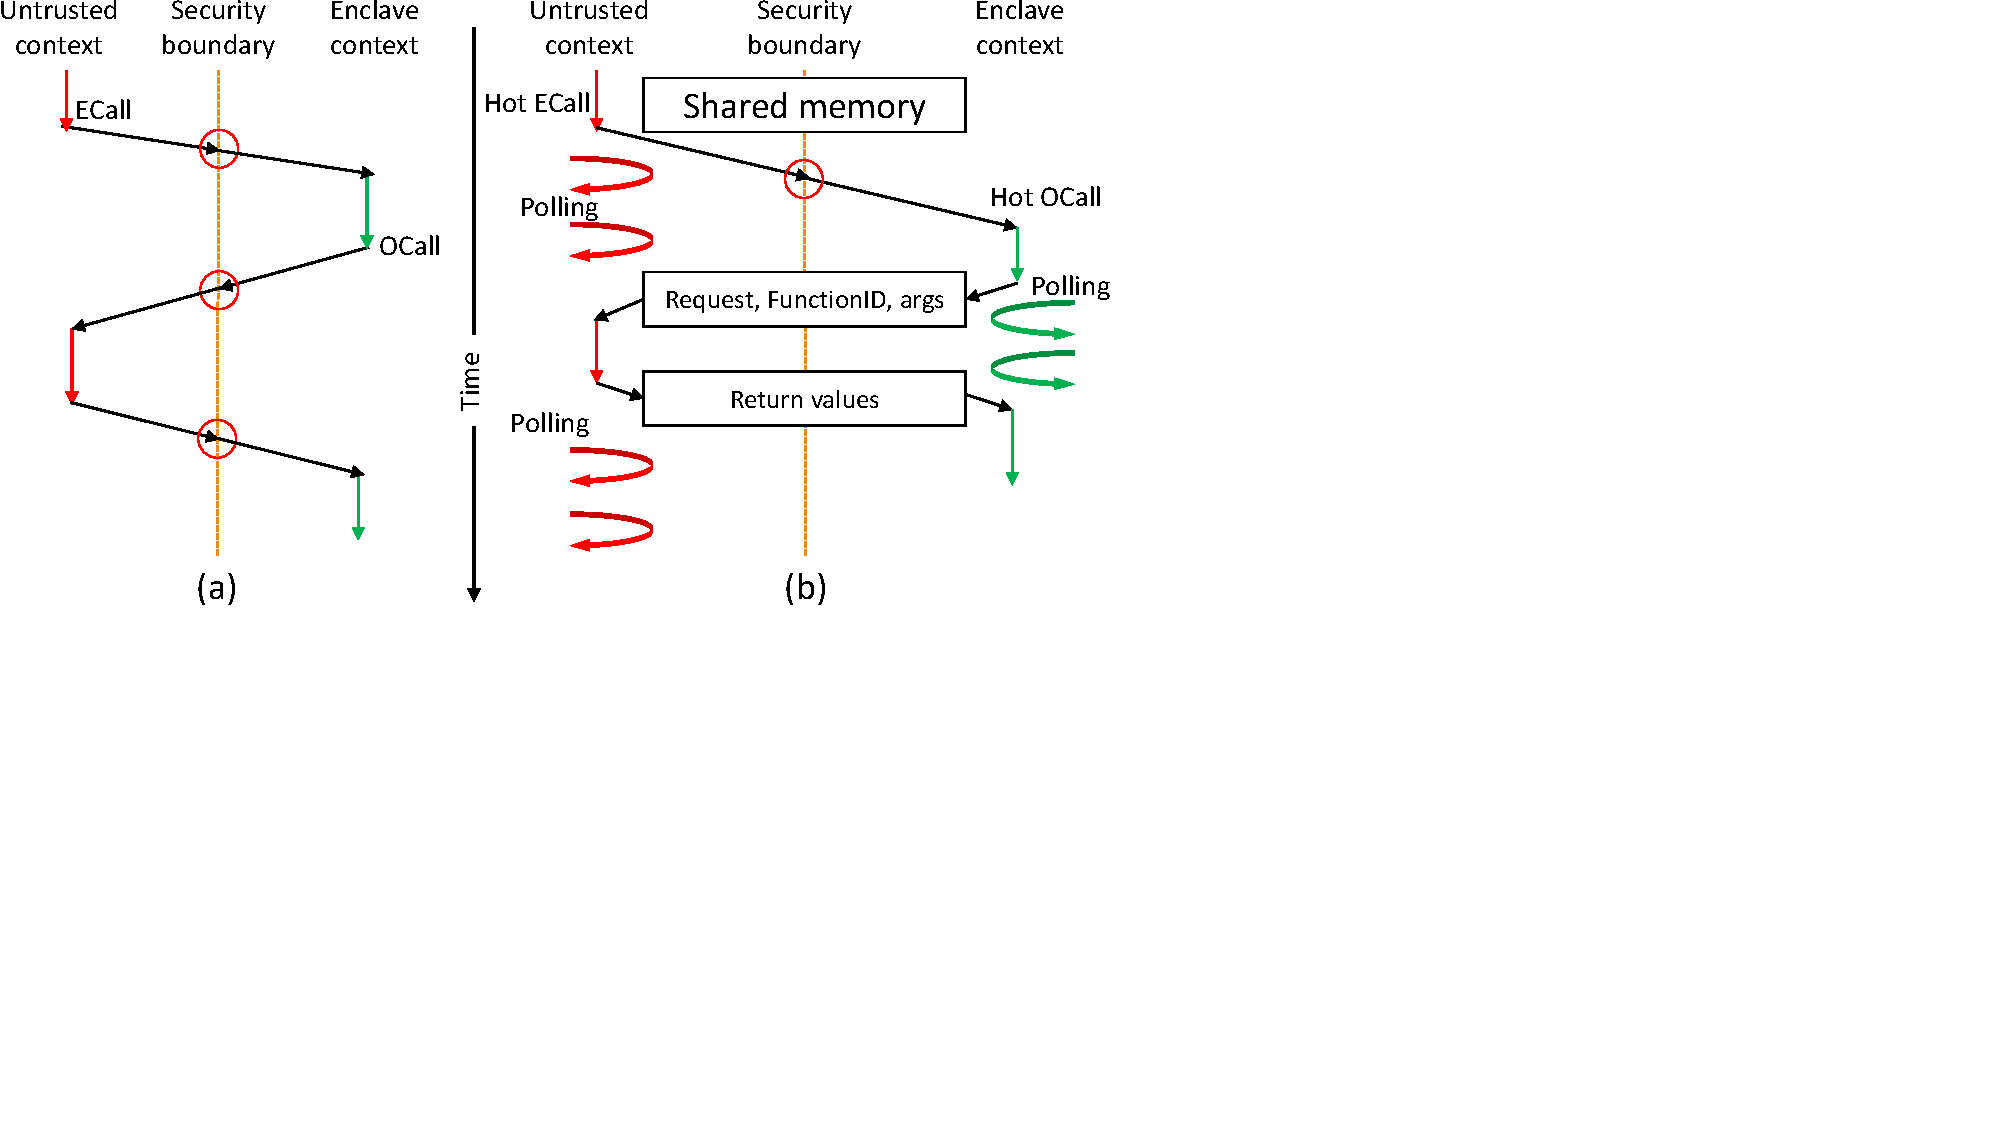
\includegraphics[trim={0 9cm 15cm 0}, clip, width=\linewidth]{chapters/ProximiTEE/images_new/hotcalls.pdf}
    \caption[Program flow control for Intel SGX SDK vs HotCalls]{\textbf{Program flow control for (a) Intel SGX SDK vs (b) HotCalls.} The figure shows efficient communication between the untrusted application and the trusted enclave. In Intel SGX SDK, the developers need to rely on the \texttt{ECALL} and \texttt{OCALL} to context switch to and from the enclave. In HotCalls, the application and the enclave communication over the shared memory -- eliminating the need for time-consuming context switch.}
    \label{fig:hotcalls}
\end{figure}

\myparagraph{HotCalls} ECalls and OCalls are expensive. To overcome this, Weisse et al. propose a solution called HotCalls~\cite{weisse2017regaining}. The key concept is that instead of having one thread that calls ECall and OCall functions, thereby entering and leaving the enclave context, we have two threads: one running in an untrusted context, the other in the enclave context. Both threads have access to a shared data structure (SDS) in unencrypted memory. We designate one thread to be the responder, while the other is the requester. The responder is dedicated to polling the SDS. The requester issues a request by passing its arguments to the SDS, including an ID of the function he wants to call. The responder detects these requests and calls the function indicated by the ID. Upon completion, it writes any results back to the SDS. The requester polls the SDS until the responder has indicated completion. It can then read the return values from the SDS. In order to have HotOCalls, the application thread acts as a responder, and the enclave thread is the requester. This is what we have used in our implementation. For HotECalls, the roles are reversed. Figure~\ref{fig:hotcalls}(a) shows the control flow of a normal OCall. Figure~\ref{fig:hotcalls}(b) shows the control flow of the same function call but using HotCalls.

We evaluate the effect of incorporating HotCalls with our simulated client. When using SDK calls, we get an average of 12.8$\mu$s per round. When using HotCalls, we can reduce it to 2.7$\mu$s per round, an improvement of a factor of 4.7.